\section{Mikołaj Mazur}

\subsection{Isaac Newton}
\hspace{\parindent}\textbf{Isaac Newton} urodził się \textbf{25 grudnia 1642 roku w Woolsthorpe, Anglia}. Był jednym z najważniejszych \textbf{fizyków, matematykiem i astronomem}, który położył podwaliny pod klasyczną mechanikę. Jego odkrycia w dziedzinie matematyki, jak i fizyki, mają ogromne znaczenie dla dzisiejszej nauki. Newton jest szczególnie znany z \textbf{trzech zasad dynamiki}, które w połączeniu z jego \textbf{prawem powszechnego ciążenia}, zrewolucjonizowały sposób, w jaki ludzie postrzegają ruch ciał w przestrzeni. \par
\hspace{\parindent}Newton był także wynalazcą \textbf{rachunku różniczkowego}, co stało się jednym z największych osiągnięć matematycznych jego czasów. Jego prace na temat optyki, w których dowiódł, że \textbf{światło białe} jest \textbf{mieszaniną wszystkich kolorów}, miały wielkie znaczenie w rozwoju tej dziedziny.

\subsection{Prawo Powszechnego Ciążenia}

\hspace{\parindent}Jednym z najsłynniejszych wyrażeń matematycznych stworzonych przez Newtona jest \textbf{prawo powszechnego ciążenia}, które można zapisać jako:

\[
F = G \frac{m_1 m_2}{r^2}
\]

gdzie:
- \( F \) to siła grawitacji,
- \( G \) to stała grawitacyjna,
- \( m_1 \) i \( m_2 \) to masy dwóch ciał,
- \( r \) to odległość między środkami tych ciał.

\begin{figure}[h]
    \centering
    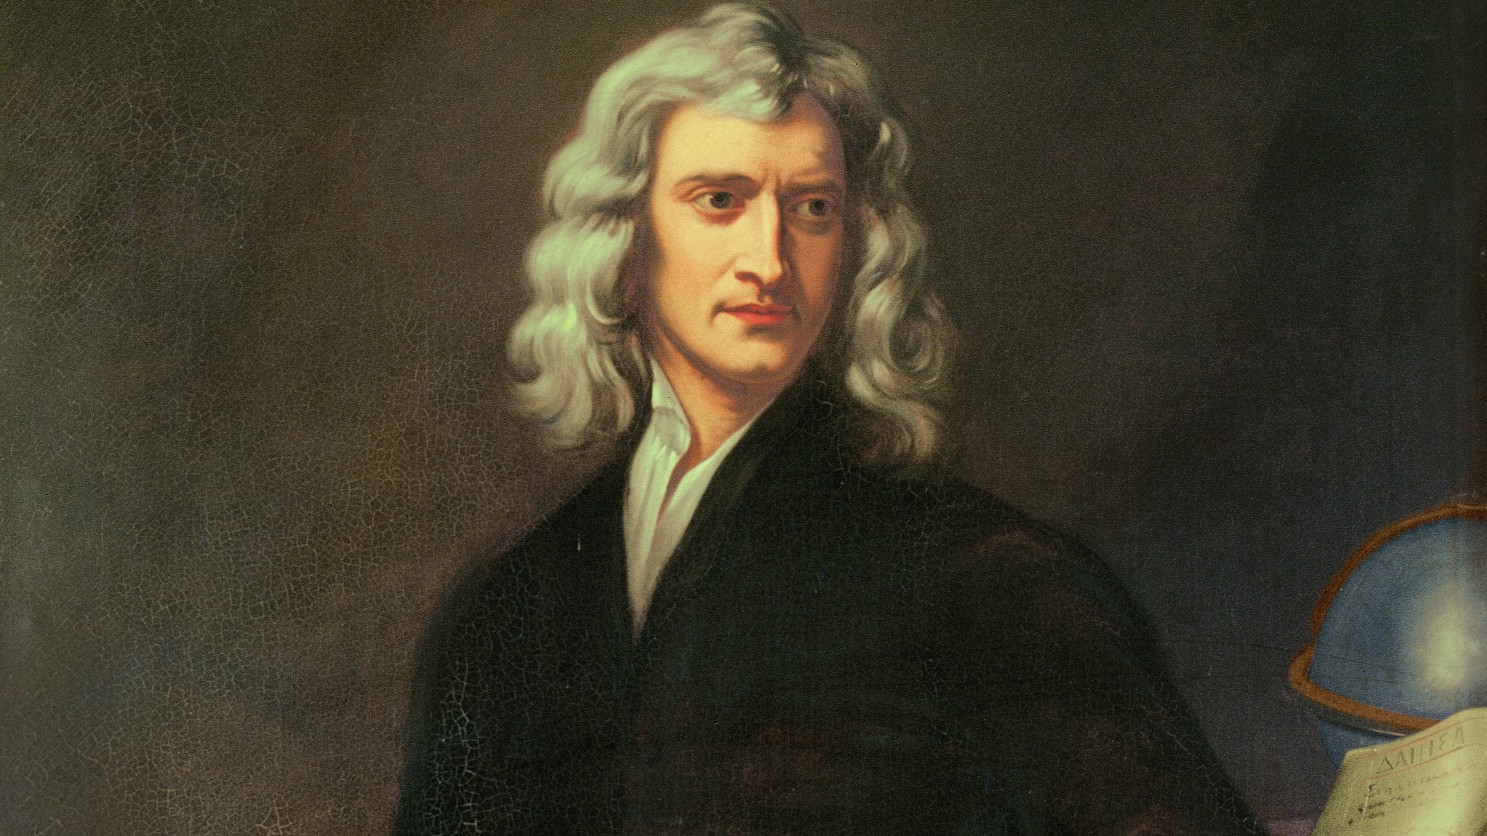
\includegraphics[width=0.5\textwidth]{pictures/newton.jpg}
    \caption{Isaac Newton}
    \label{fig:newton}
\end{figure}
\par

\subsection{Najważniejsze Daty, Odkrycia i Wydarzenia}

Najważniejszymi osiągnięcia Newtona (lista I):

\begin{enumerate}
    \item Opracowanie trzech zasad dynamiki
    \item Sformułowanie prawa powszechnego ciążenia
    \item Wynalezienie rachunku różniczkowego
    \item Badania nad optyką
\end{enumerate}

Najważniejszymi osiągnięcia Newtona (lista II):

\begin{itemize}
    \renewcommand\labelitemi{--}
    \item Zasady dynamiki
    \item Prawo powszechnego ciążenia
    \item Optyka
\end{itemize}


Najważniejsze daty z życia Newtona:

\begin{table}[h]
    \centering
    \begin{tabular}{|c|c|}
    \hline
    Rok & Wydarzenie \\
    \hline
    1642 & Urodziny Newtona \\
    \hline
    1687 & Publikacja "Philosophiæ Naturalis Principia Mathematica" \\
    \hline
    1705 & Newton otrzymuje tytuł szlachecki \\
    \hline
    1727 & Śmierć Newtona \\
    \hline
    \end{tabular}
    \caption{Najważniejsze daty z życia Isaaca Newtona}
    \label{tab:newton}
\end{table}
